\documentclass[conference]{IEEEtran}
\IEEEoverridecommandlockouts

\usepackage[utf8]{inputenc}
\usepackage[spanish]{babel}
\usepackage{amsmath,amssymb}
\usepackage{graphicx}
\usepackage{booktabs}
\usepackage{hyperref}
\usepackage{xcolor}
\usepackage{subcaption}
\usepackage{multirow}

\graphicspath{{./}}

\title{Destilado de Modelos para Detección de Anomalías\\
\large Proyecto II --- Curso de Inteligencia Artificial\\
Instituto Tecnológico de Costa Rica}

\author{
  \IEEEauthorblockN{Allan B}
  \IEEEauthorblockA{Escuela de Ingeniería en Computación\\
  Instituto Tecnológico de Costa Rica\\
  adbyb.es@gmail.com\\
  \url{https://github.com/AllanDBB/nomaly-detection-distillation}}
}

\begin{document}
\maketitle

% ─────────────────────────────────────────────────────────────────────────────
\begin{abstract}
Este trabajo valida la hipótesis de que el destilado de conocimiento permite
comprimir modelos de gran escala en arquitecturas más eficientes sin sacrificar
capacidad para tareas complejas. Se implementan tres modelos para detección de
anomalías sobre el dataset MVTec AD (10 clases): un clasificador CNN entrenado
desde cero (Modelo A), el mismo clasificador entrenado mediante destilado
\textit{teacher-student} usando ResNet-18 preentrenado como teacher (Modelo B),
y un autoencoder U-Net (Modelo C). Los embeddings de cada modelo se utilizan
para detectar anomalías mediante distancia de Mahalanobis; el Modelo C también
usa el error de reconstrucción como señal directa de anomalía. Se aplica DBSCAN
sobre representaciones reducidas con PCA y t-SNE para análisis no supervisado de
outliers. Los resultados muestran que el Modelo B supera al Modelo A en AUROC
(0.453 vs. 0.365), validando la hipótesis del destilado, mientras que el error
de reconstrucción del U-Net obtiene el mayor AUROC global (0.490). En análisis
DBSCAN, t-SNE produce separaciones notablemente superiores a PCA en todos los
modelos, con F1 $\approx$ 0.86 para el Modelo A.
\end{abstract}

% ─────────────────────────────────────────────────────────────────────────────
\section{Introducción}

La detección de anomalías en entornos industriales es un problema crítico donde
los modelos deben identificar defectos sin haber sido entrenados con ejemplos
anómalos. El \textit{transfer learning} y el destilado de modelos ofrecen una
alternativa viable para obtener representaciones latentes de alta calidad con
arquitecturas compactas.

El objetivo de este proyecto es validar experimentalmente si un modelo student
entrenado mediante destilado de ResNet-18 produce embeddings superiores a los
de un modelo entrenado desde cero, aplicados a la detección de anomalías en
el dataset MVTec AD \cite{bergmann2019mvtec}.

Las contribuciones principales son:
\begin{itemize}
  \item Implementación de tres modelos con PyTorch Lightning e integración con
        Hydra y WandB para gestión reproducible de experimentos.
  \item Evaluación cuantitativa de detección de anomalías mediante distancia
        de Mahalanobis por clase con umbral basado en percentil.
  \item Análisis no supervisado con DBSCAN sobre espacios latentes reducidos
        mediante PCA y t-SNE.
\end{itemize}

% ─────────────────────────────────────────────────────────────────────────────
\section{Dataset}

Se utiliza el dataset MVTec AD \cite{bergmann2019mvtec}, un benchmark estándar
para detección de anomalías industriales. Se seleccionaron 10 clases:
\textit{bottle, cable, capsule, carpet, grid, hazelnut, leather, metal\_nut,
pill} y \textit{screw}.

Cada clase contiene imágenes de entrenamiento exclusivamente normales, e imágenes
de prueba tanto normales como defectuosas. El entrenamiento de todos los modelos
se realiza \textbf{únicamente con imágenes sin defectos}, siguiendo el paradigma
de detección de anomalías unilateral (\textit{one-class}).

Las imágenes se redimensionan a $256 \times 256$ píxeles. Se aplica
\textit{data augmentation} durante el entrenamiento (flip horizontal/vertical,
jitter de brillo y contraste) y normalización con estadísticas ImageNet.

% ─────────────────────────────────────────────────────────────────────────────
\section{Modelos}

\subsection{Arquitectura base CNN}

El backbone CNN sigue la estructura de las primeras tres etapas de ResNet-18
\cite{he2016deep}: \texttt{conv1} ($7\times7$, stride 2 + MaxPool),
\texttt{conv2\_x} (2 bloques BasicBlock de 64 canales) y \texttt{conv3\_x}
(2 bloques BasicBlock de 128 canales con stride 2). Para una entrada de
$3\times256\times256$, la salida tras \texttt{conv3\_x} es $128\times32\times32$.
Un \textit{global average pool} produce el \textbf{embedding de 128 dimensiones}
usado para detección de anomalías.

Un clasificador FC (128 $\rightarrow$ \textit{hidden\_dim} $\rightarrow$ 10)
proporciona la señal de supervisión durante el entrenamiento.

\subsection{Modelo A — CNN desde cero}

El Modelo A inicializa todos los pesos aleatoriamente y minimiza la
\textit{cross-entropy} sobre las 10 clases normales. La tarea de clasificación
fuerza al modelo a aprender representaciones discriminativas de cada categoría
normal, lo que produce embeddings útiles para detectar desviaciones anómalas.

\subsection{Modelo B — Destilado Teacher-Student}

El Modelo B emplea la técnica de destilado de conocimiento
\cite{hinton2015distilling} con:

\begin{itemize}
  \item \textbf{Teacher:} ResNet-18 preentrenado en ImageNet (pesos congelados).
  \item \textbf{Student:} Misma arquitectura CNN base que el Modelo A.
\end{itemize}

Se utiliza \textbf{destilado a nivel de características} (\textit{feature-level
distillation}): las activaciones intermedias del student y del teacher se
comparan tras un \textit{global average pool}. Dado que el student replica
exactamente \texttt{layer1} y \texttt{layer2} de ResNet-18, las dimensiones
coinciden naturalmente (64-dim y 128-dim respectivamente).

La función de pérdida combinada es:
\begin{equation}
  \mathcal{L} = \alpha \cdot \mathcal{L}_{CE} + \beta \cdot \mathcal{L}_{feat_1}
              + \gamma \cdot \mathcal{L}_{feat_2}
\end{equation}
donde $\mathcal{L}_{CE}$ es la \textit{cross-entropy} con etiquetas duras y
$\mathcal{L}_{feat_i}$ es el MSE entre las activaciones del student y el teacher
en la $i$-ésima capa convolucional.

\subsection{Modelo C — Autoencoder U-Net}

El Modelo C es un autoencoder basado en U-Net \cite{ronneberger2015unet} que
reconstruye las imágenes normales de entrenamiento. El encoder aplica 4 bloques
DoubleConv + MaxPool (64$\rightarrow$128$\rightarrow$256$\rightarrow$512 canales),
el bottleneck expande a 1024 canales, y el decoder espeja el encoder con conexiones
de salto (\textit{skip connections}).

El \textbf{embedding} se obtiene proyectando el bottleneck mediante
$\text{GAP} \rightarrow \text{Linear}(1024, d)$. El error de reconstrucción MSE
también sirve como señal de anomalía alternativa.

\subsection{Implementación}

Todos los modelos se implementan con \textbf{PyTorch Lightning} usando
\texttt{LightningModule} y \texttt{LightningDataModule}. Los hiperparámetros
se gestionan con \textbf{Hydra} y los experimentos se registran en \textbf{WandB}.
Se usa \textit{EarlyStopping} (paciencia de 10 épocas, máximo 50--60 épocas)
para prevenir overfitting.

% ─────────────────────────────────────────────────────────────────────────────
\section{Diseño Experimental}

Cada modelo se entrena con \textbf{3 configuraciones de hiperparámetros} distintas.
La Tabla~\ref{tab:hyperparams} resume las configuraciones evaluadas. Para el
Modelo B, $\alpha$, $\beta$ y $\gamma$ ponderan $\mathcal{L}_{CE}$,
$\mathcal{L}_{feat_1}$ y $\mathcal{L}_{feat_2}$ respectivamente.
Para el Modelo C, \textit{f} indica los canales de cada bloque encoder y
\textit{emb} la dimensión del espacio latente.

\begin{table*}[t]
\centering
\caption{Configuraciones de hiperparámetros evaluadas por modelo}
\label{tab:hyperparams}
\begin{tabular}{llccccc}
\toprule
Modelo & Config & LR & HD / emb & Canales (f) & BS & $\alpha/\beta/\gamma$ \\
\midrule
\multirow{3}{*}{A (Scratch)}
  & C1 & $10^{-3}$       & 256 & —                  & 32 & — \\
  & C2 & $5\!\times\!10^{-4}$ & 512 & —             & 32 & — \\
  & C3 & $10^{-4}$       & 128 & —                  & 64 & — \\
\midrule
\multirow{3}{*}{B (Destilado)}
  & C1 & $10^{-3}$       & 256 & —                  & 32 & 0.5/0.3/0.2 \\
  & C2 & $5\!\times\!10^{-4}$ & 256 & —             & 32 & 0.7/0.2/0.1 \\
  & C3 & $10^{-4}$       & 512 & —                  & 64 & 0.3/0.4/0.3 \\
\midrule
\multirow{3}{*}{C (U-Net)}
  & C1 & $10^{-4}$       & 256 & [64,128,256,512]   &  4 & — \\
  & C2 & $10^{-4}$       & 128 & [32,64,128,256]    &  8 & — \\
  & C3 & $5\!\times\!10^{-5}$ & 512 & [64,128,256,512] & 4 & — \\
\bottomrule
\end{tabular}
\end{table*}

% ─────────────────────────────────────────────────────────────────────────────
\section{Detección de Anomalías}

\subsection{Distancia de Mahalanobis}

Para cada modelo se extraen los embeddings del conjunto de validación (imágenes
normales únicamente). Se estima una distribución gaussiana por clase:
\begin{equation}
  \boldsymbol{\mu}_c = \frac{1}{N_c}\sum_{i=1}^{N_c} \mathbf{z}_i, \quad
  \boldsymbol{\Sigma}_c = \frac{1}{N_c-1}\sum_{i=1}^{N_c}(\mathbf{z}_i - \boldsymbol{\mu}_c)(\mathbf{z}_i - \boldsymbol{\mu}_c)^\top
\end{equation}

Para una imagen de prueba con embedding $\mathbf{z}_{test}$, el score de anomalía
es la distancia mínima a cualquier distribución de clase:
\begin{equation}
  s(\mathbf{z}_{test}) = \min_c \sqrt{(\mathbf{z}_{test} - \boldsymbol{\mu}_c)^\top
  \boldsymbol{\Sigma}_c^{-1} (\mathbf{z}_{test} - \boldsymbol{\mu}_c)}
\end{equation}

El umbral de clasificación se fija en el percentil 95 de los scores de validación.

\subsection{Error de Reconstrucción (Modelo C)}

Para el autoencoder U-Net, el error de reconstrucción por imagen también sirve
como score de anomalía:
\begin{equation}
  s_{recon}(\mathbf{x}) = \|\mathbf{x} - \hat{\mathbf{x}}\|_F^2
\end{equation}
donde $\hat{\mathbf{x}}$ es la reconstrucción del modelo.

% ─────────────────────────────────────────────────────────────────────────────
\section{Resultados}

\subsection{Entrenamiento y overfitting}

Las Figuras~\ref{fig:overfitting_a}, \ref{fig:overfitting_b} y
\ref{fig:overfitting_c} muestran las curvas de pérdida de entrenamiento y
validación para las 3 configuraciones de cada modelo. El área sombreada en rojo
indica el gap val$-$train; valores positivos crecientes indican overfitting.

El uso de \textit{EarlyStopping} detuvo el entrenamiento antes de las épocas
máximas en la mayoría de las configuraciones, indicando convergencia efectiva.

\begin{figure}[t]
  \centering
  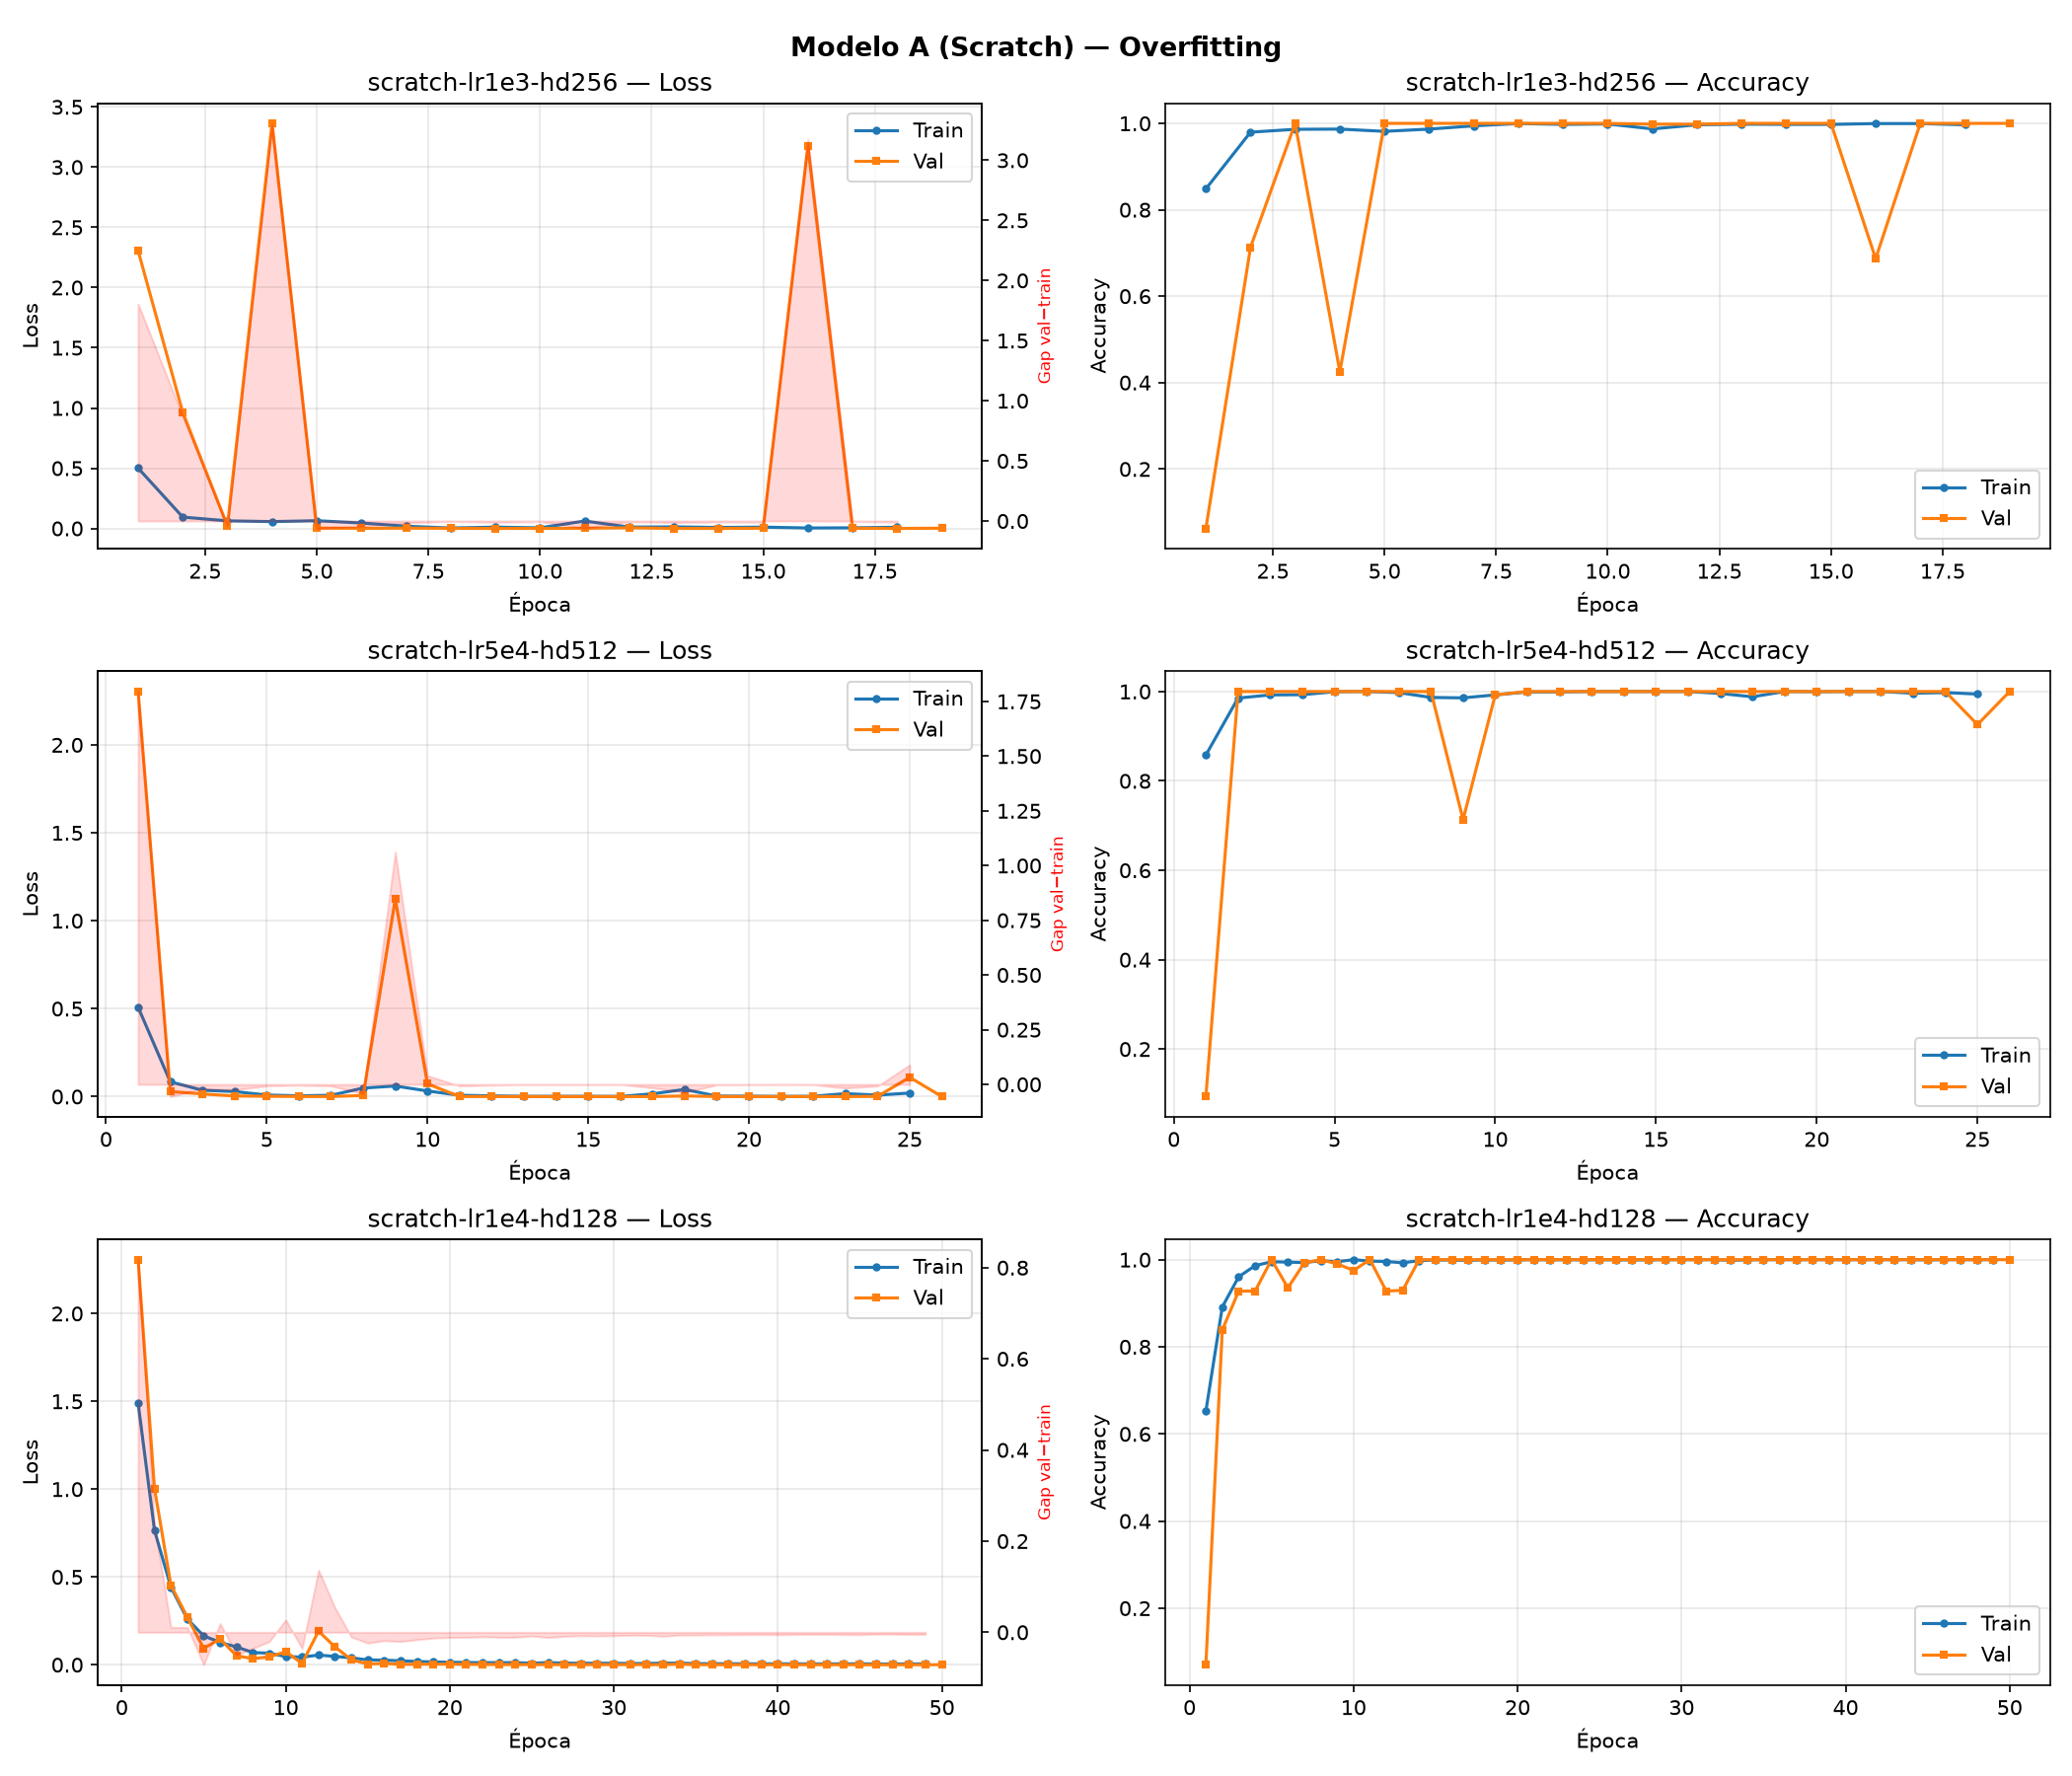
\includegraphics[width=\columnwidth]{overfitting_cnn_scratch.png}
  \caption{Curvas train/val — Modelo A (Scratch).}
  \label{fig:overfitting_a}
\end{figure}

\begin{figure}[t]
  \centering
  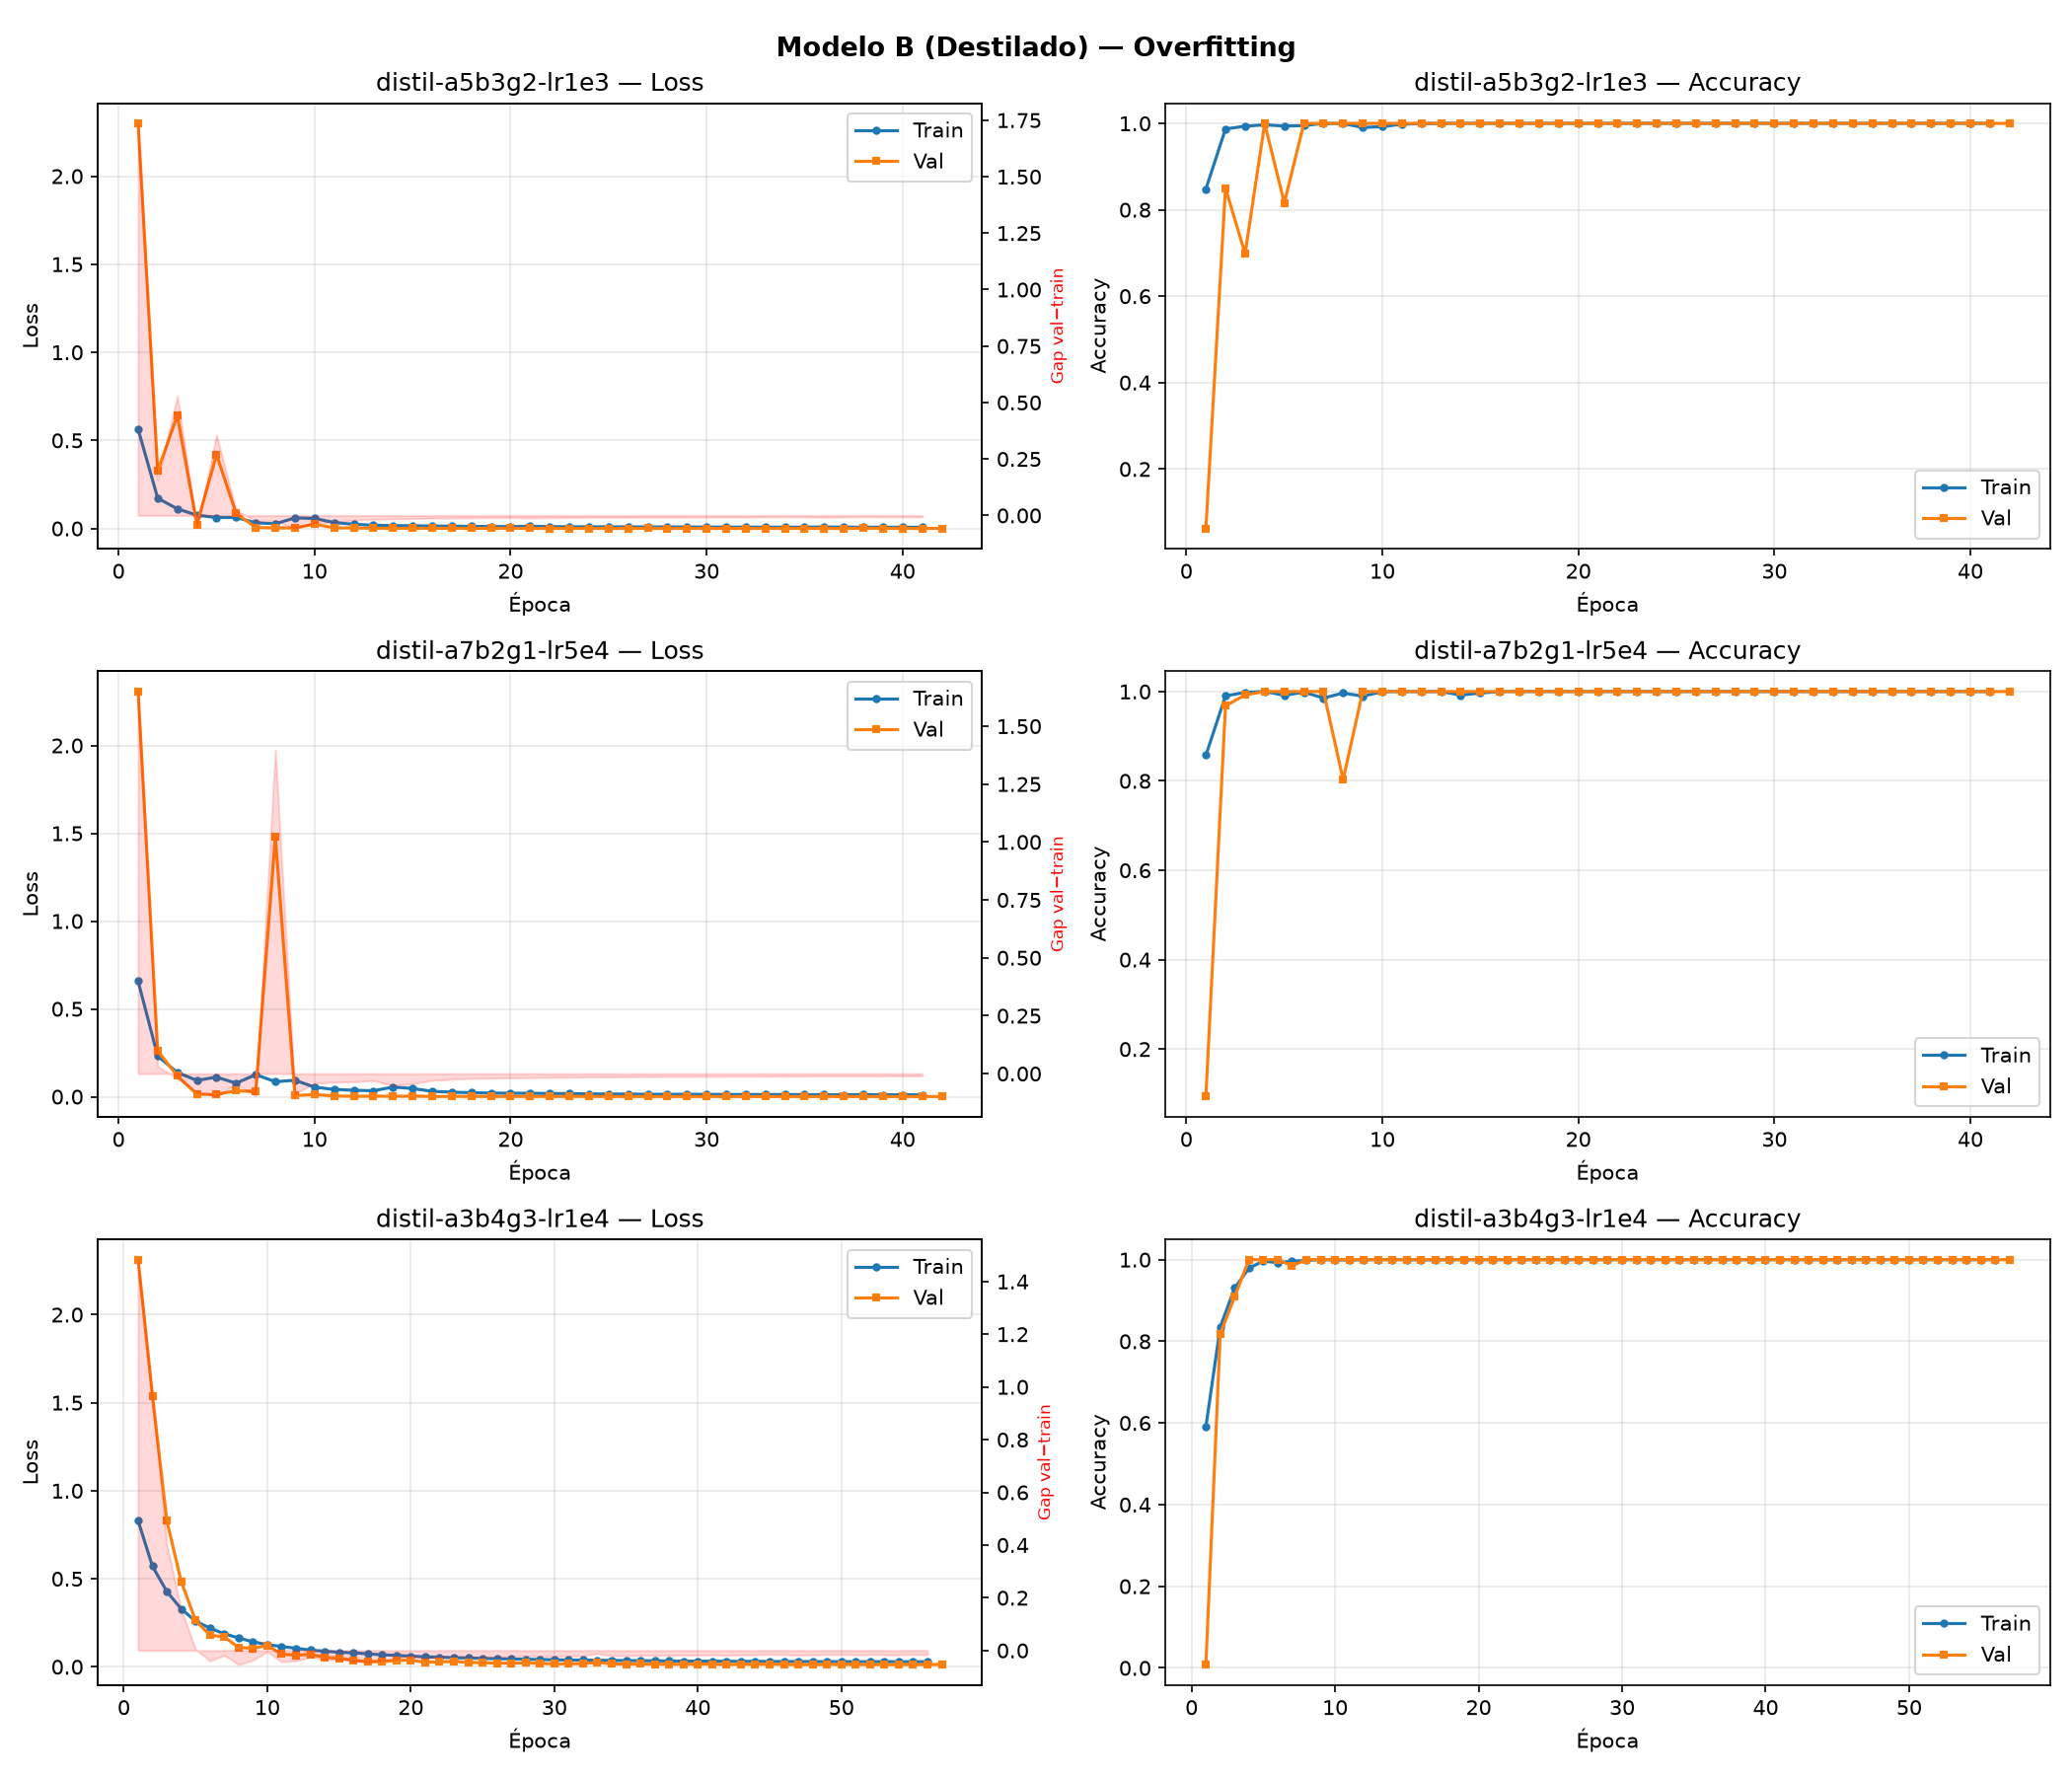
\includegraphics[width=\columnwidth]{overfitting_cnn_distilled.png}
  \caption{Curvas train/val — Modelo B (Destilado).}
  \label{fig:overfitting_b}
\end{figure}

\begin{figure}[t]
  \centering
  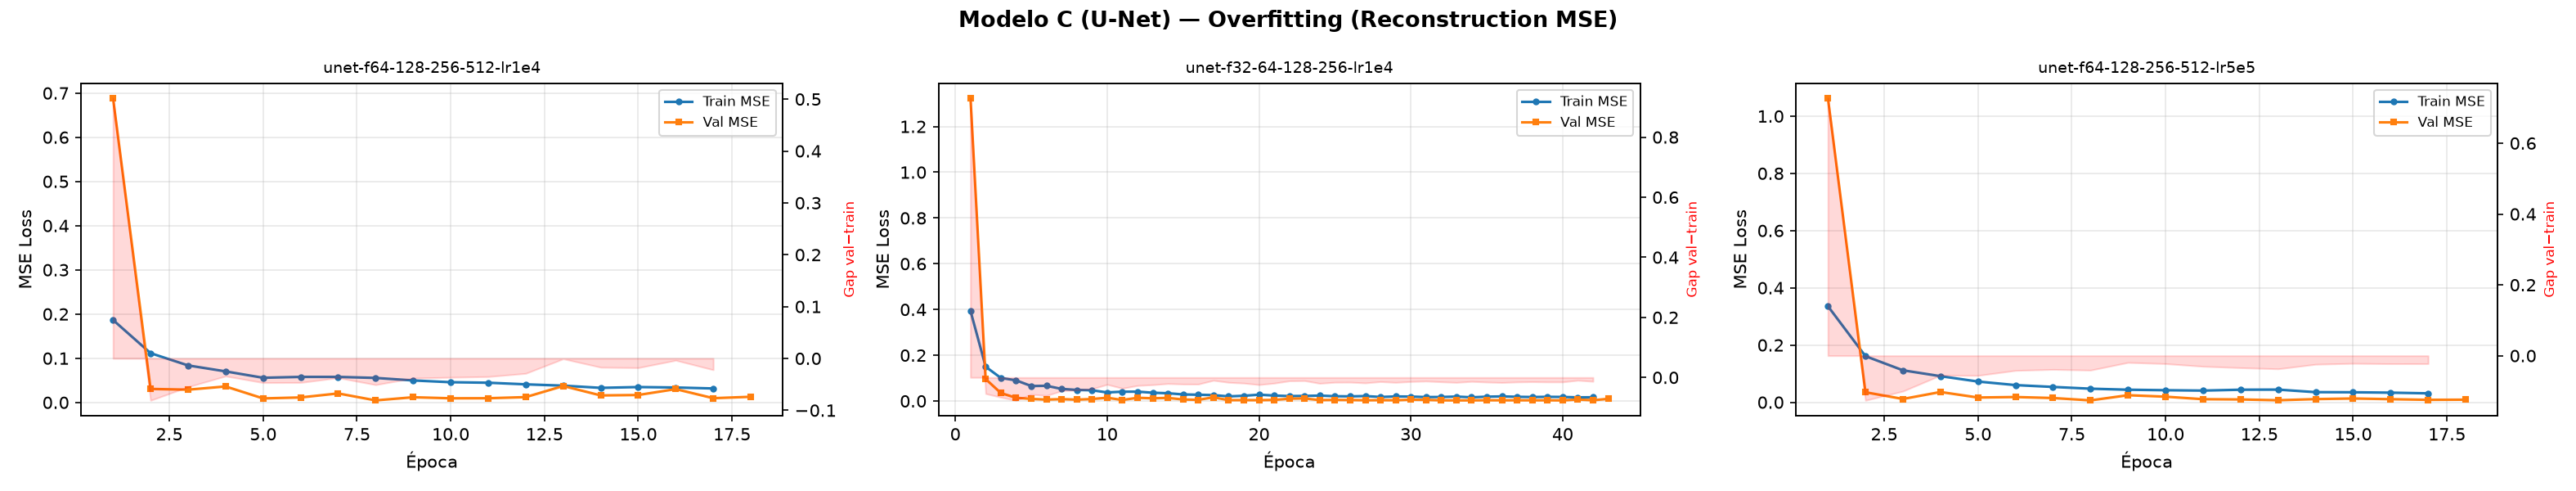
\includegraphics[width=\columnwidth]{overfitting_unet.png}
  \caption{Curvas train/val — Modelo C (U-Net, MSE de reconstrucción).}
  \label{fig:overfitting_c}
\end{figure}

\subsection{Reconstrucciones U-Net}

La Figura~\ref{fig:recon} muestra ejemplos de reconstrucción del mejor
autoencoder U-Net (Config~1, lr=$10^{-4}$, val\_loss=0.0046). Las imágenes
normales se reconstruyen con alta fidelidad, mientras que las anomalías
producen errores de reconstrucción elevados que sirven como señal de detección.

\begin{figure}[t]
  \centering
  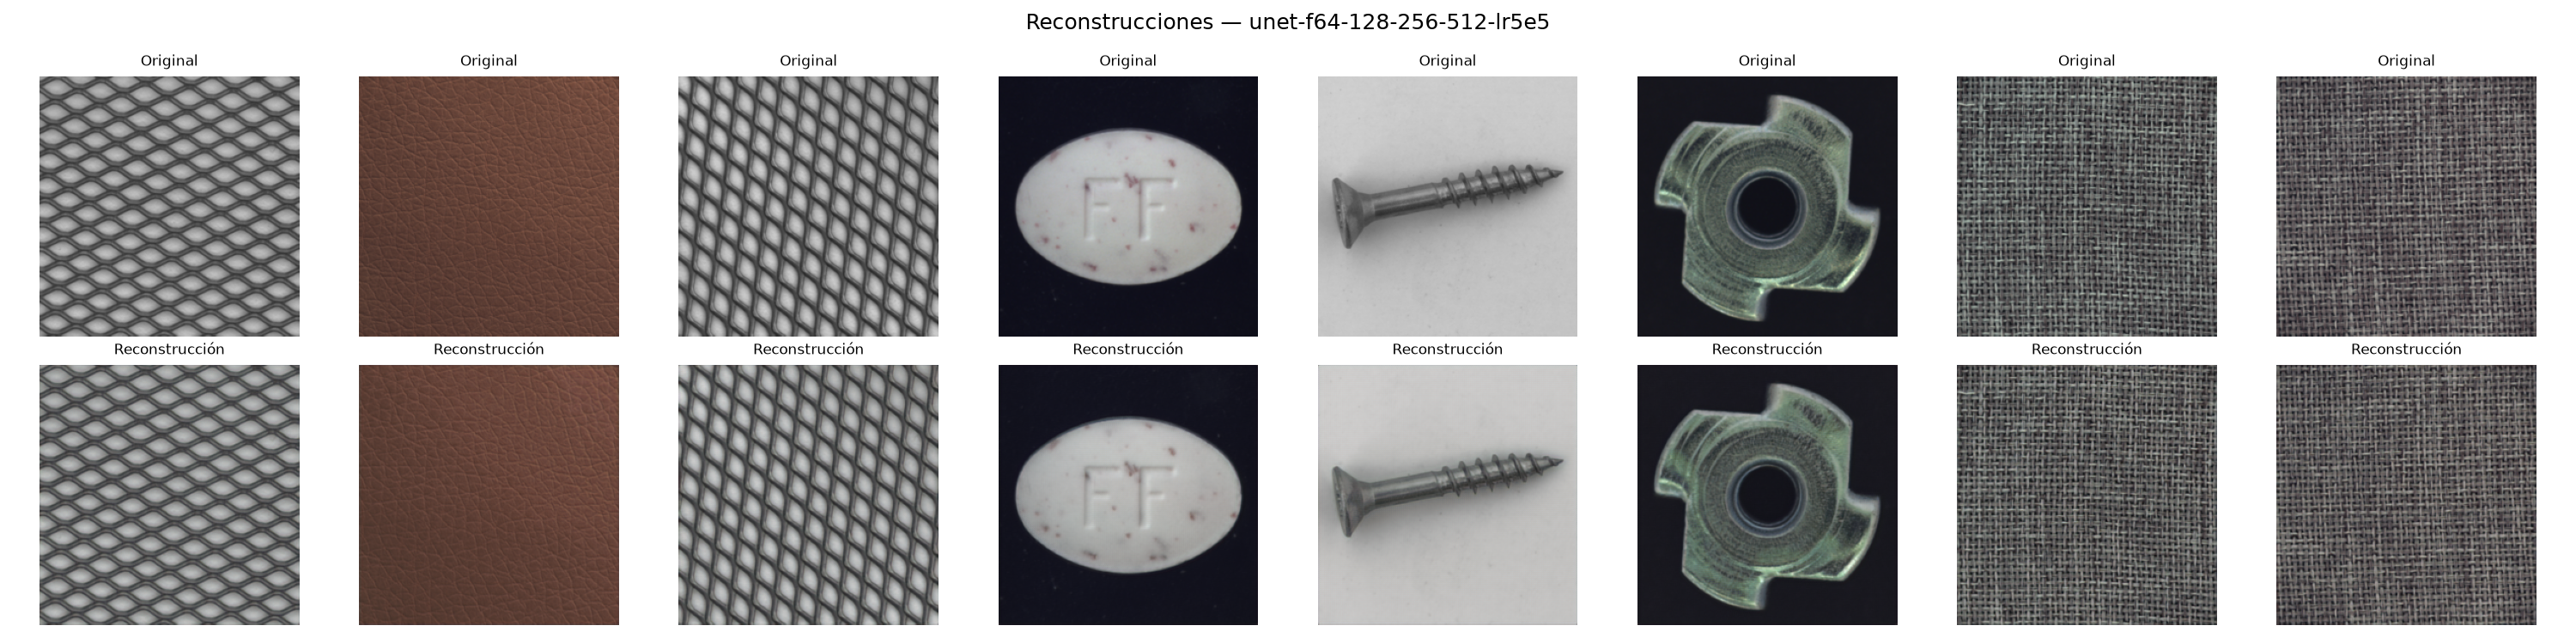
\includegraphics[width=\columnwidth]{unet_reconstructions.png}
  \caption{Originales (arriba) vs. reconstrucciones U-Net (abajo) sobre imágenes de validación.}
  \label{fig:recon}
\end{figure}

\subsection{Detección de anomalías}

La Tabla~\ref{tab:anomaly_results} compara los mejores modelos de cada tipo
en la tarea de detección de anomalías. El score de anomalía con distancia de
Mahalanobis se define como la mínima distancia a cualquier distribución
gaussiana por clase \cite{lee2018simple}.

\begin{table}[t]
\centering
\caption{Métricas de detección de anomalías (test set, umbral P95)}
\label{tab:anomaly_results}
\resizebox{\columnwidth}{!}{%
\begin{tabular}{lcccc}
\toprule
Modelo & AUROC & F1 & Prec. & Recall \\
\midrule
A — Scratch (Mahal.)   & 0.365 & 0.173 & 0.711 & 0.098 \\
B — Destilado (Mahal.) & 0.453 & \textbf{0.230} & \textbf{0.805} & \textbf{0.134} \\
C — U-Net (Mahal.)     & 0.413 & 0.114 & 0.637 & 0.063 \\
C — U-Net (Recon.)     & \textbf{0.490} & 0.107 & 0.534 & 0.060 \\
\bottomrule
\end{tabular}}
\end{table}

\begin{figure}[t]
  \centering
  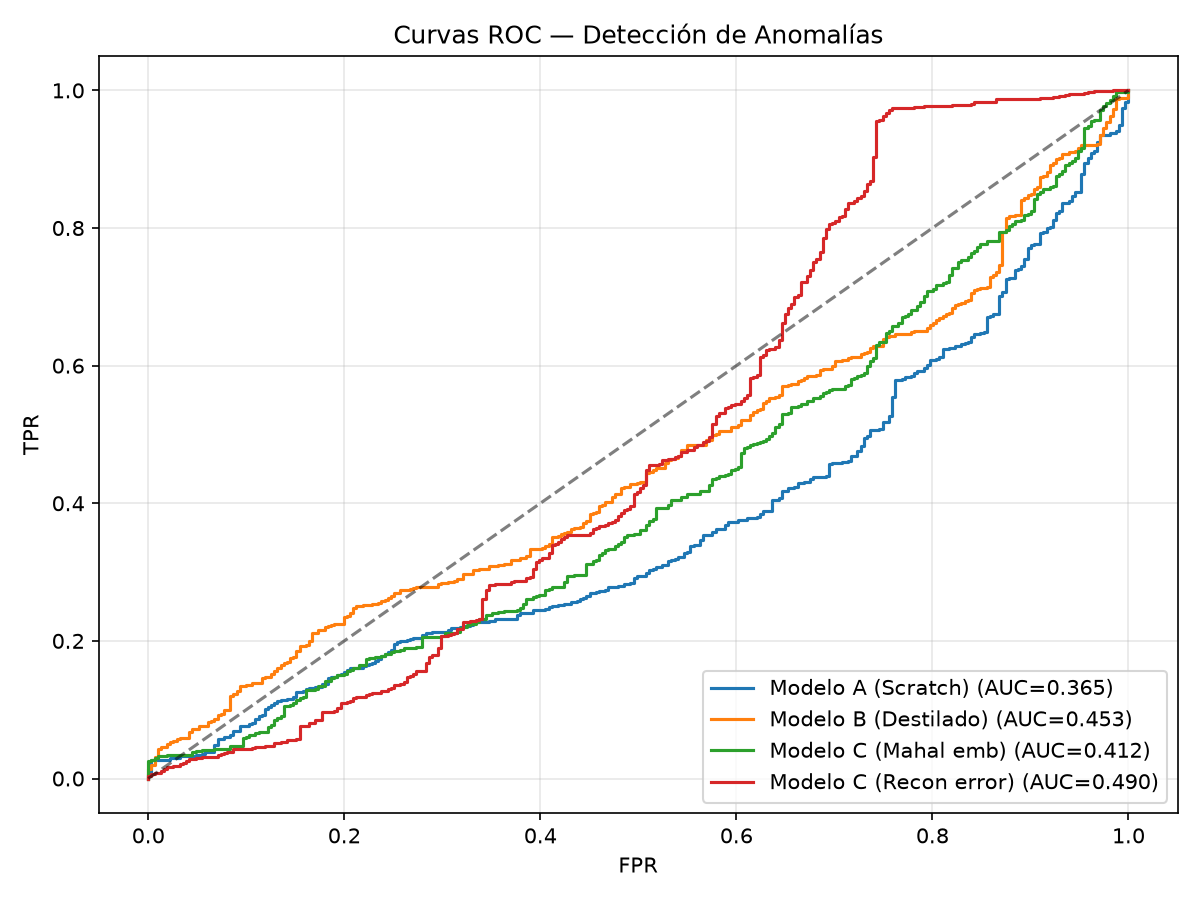
\includegraphics[width=\columnwidth]{roc_curves.png}
  \caption{Curvas ROC de los cuatro métodos de detección de anomalías.}
  \label{fig:roc}
\end{figure}

\begin{figure}[t]
  \centering
  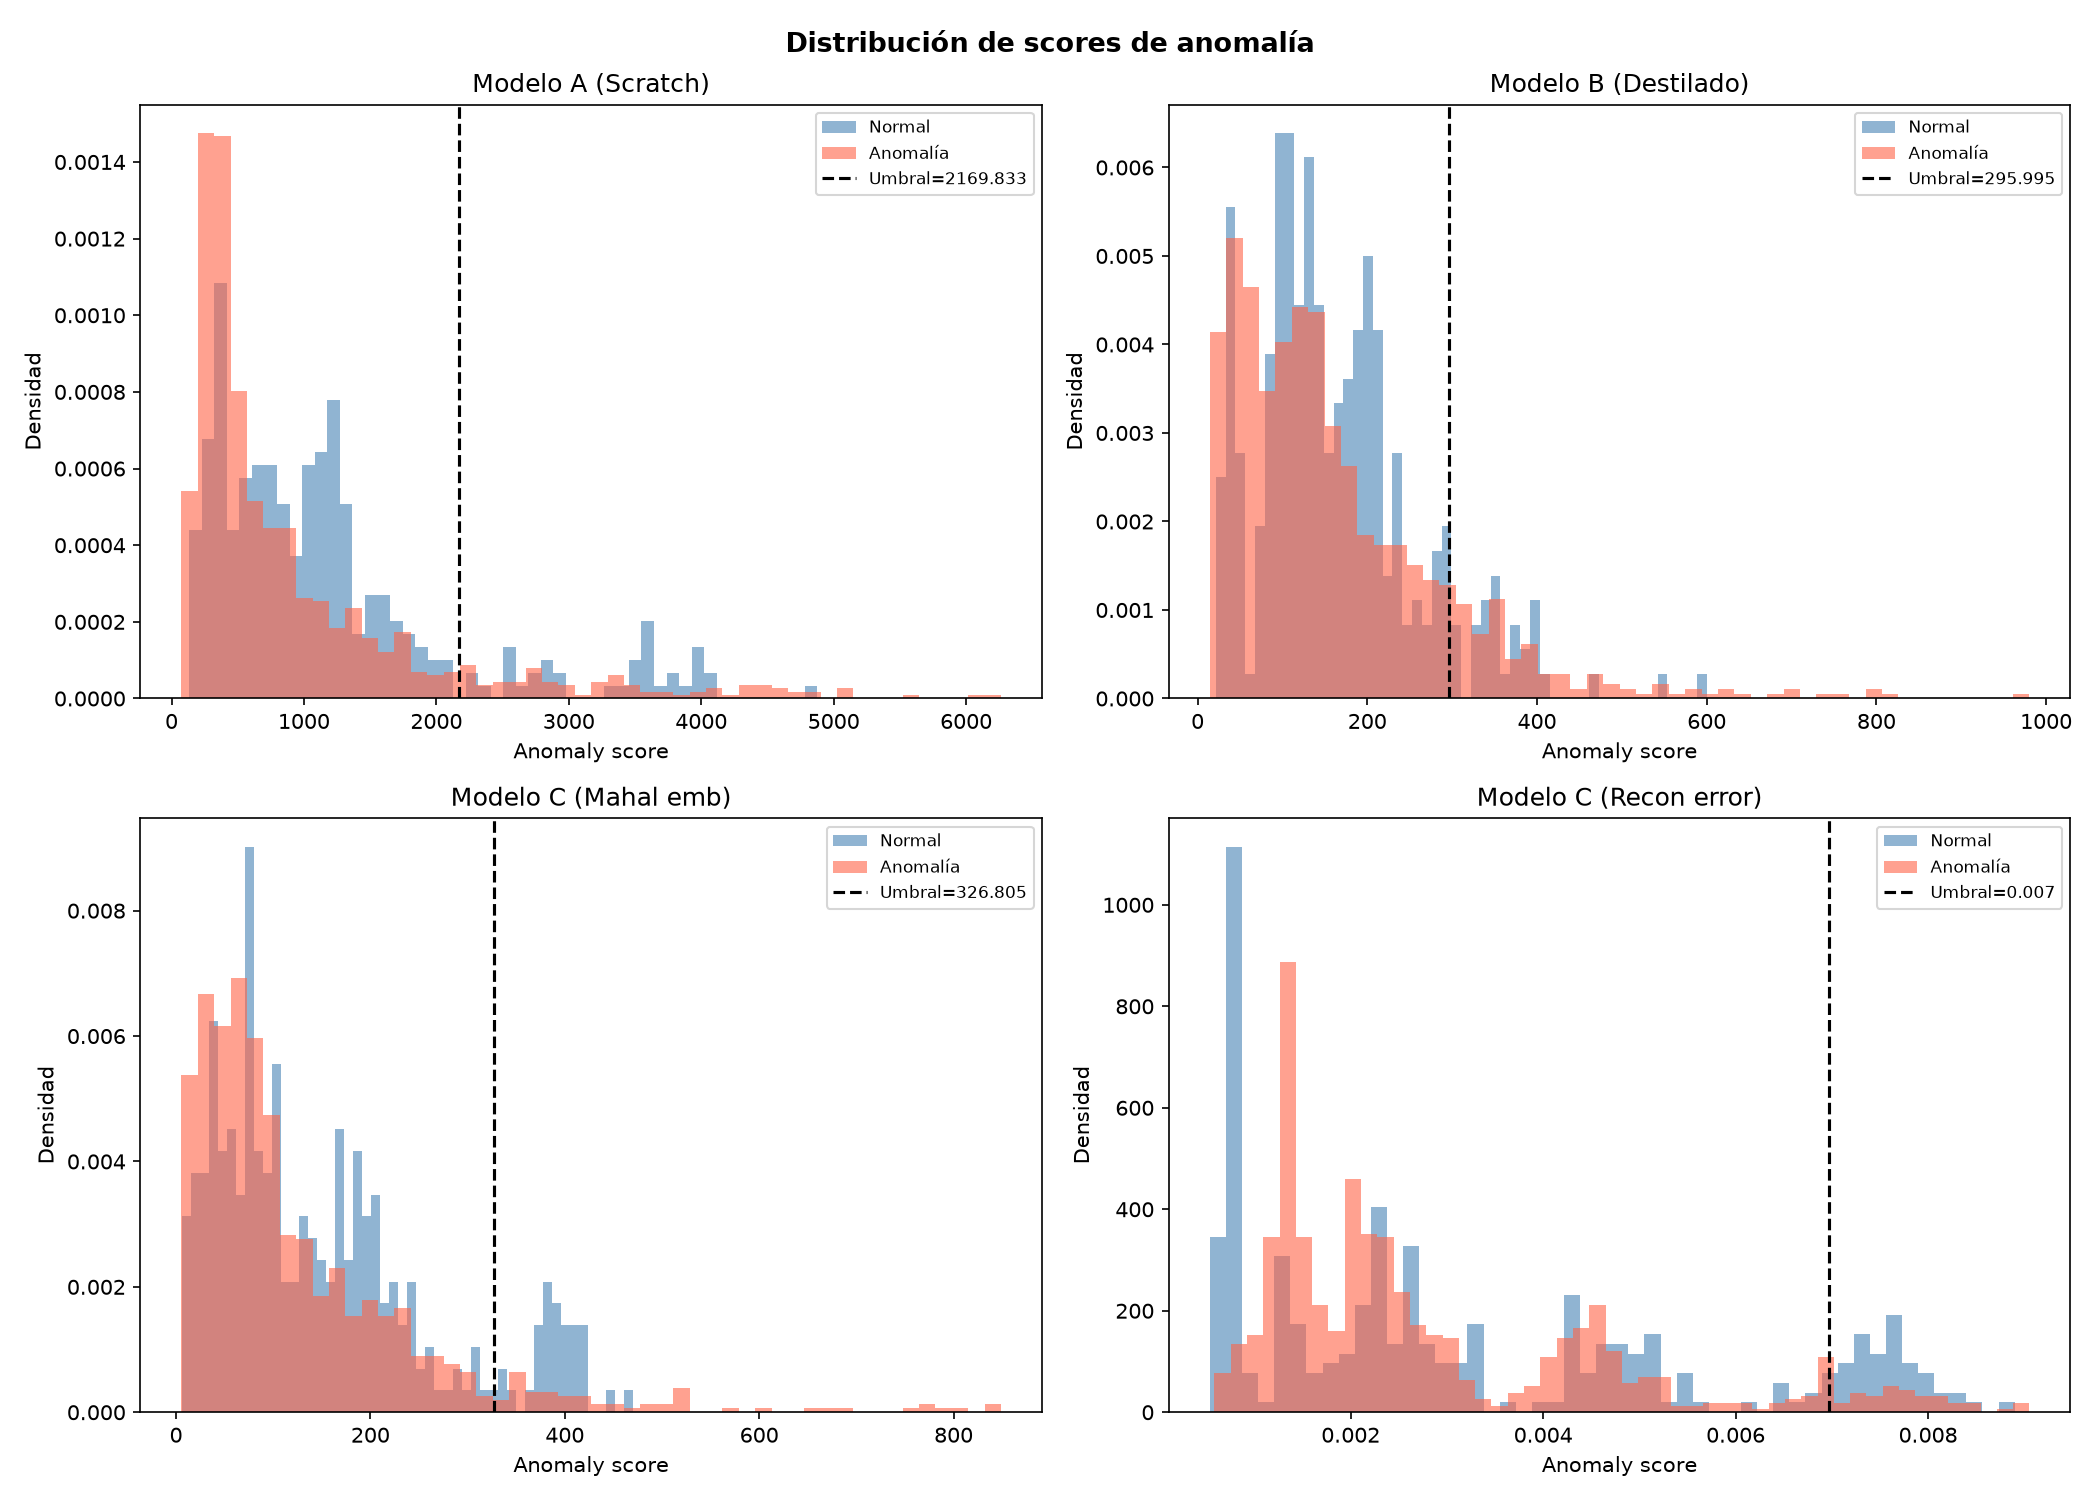
\includegraphics[width=\columnwidth]{score_distributions.png}
  \caption{Distribuciones de scores de anomalía (normal vs. anómalo).}
  \label{fig:scores}
\end{figure}

\subsection{Análisis DBSCAN}

La Tabla~\ref{tab:dbscan} resume los resultados del análisis de clustering
no supervisado con DBSCAN sobre representaciones reducidas con PCA y t-SNE.
Los puntos etiquetados como ruido (label $= -1$) corresponden a anomalías predichas.

\begin{table}[t]
\centering
\caption{Métricas DBSCAN — ruido = anomalía predicha}
\label{tab:dbscan}
\resizebox{\columnwidth}{!}{%
\begin{tabular}{llcccc}
\toprule
Modelo & Reduc. & Clusters & Noise\% & F1 & Acc. \\
\midrule
A & PCA   & 10 &  4.4\% & 0.088 & 0.278 \\
A & t-SNE &  2 & 99.1\% & \textbf{0.860} & \textbf{0.756} \\
B & PCA   &  8 &  0.0\% & 0.000 & 0.252 \\
B & t-SNE &  2 & 99.1\% & 0.855 & 0.748 \\
C & PCA   &  3 &  0.2\% & 0.006 & 0.254 \\
C & t-SNE &  4 & 94.7\% & 0.846 & 0.739 \\
\bottomrule
\end{tabular}}
\end{table}

\begin{figure}[t]
  \centering
  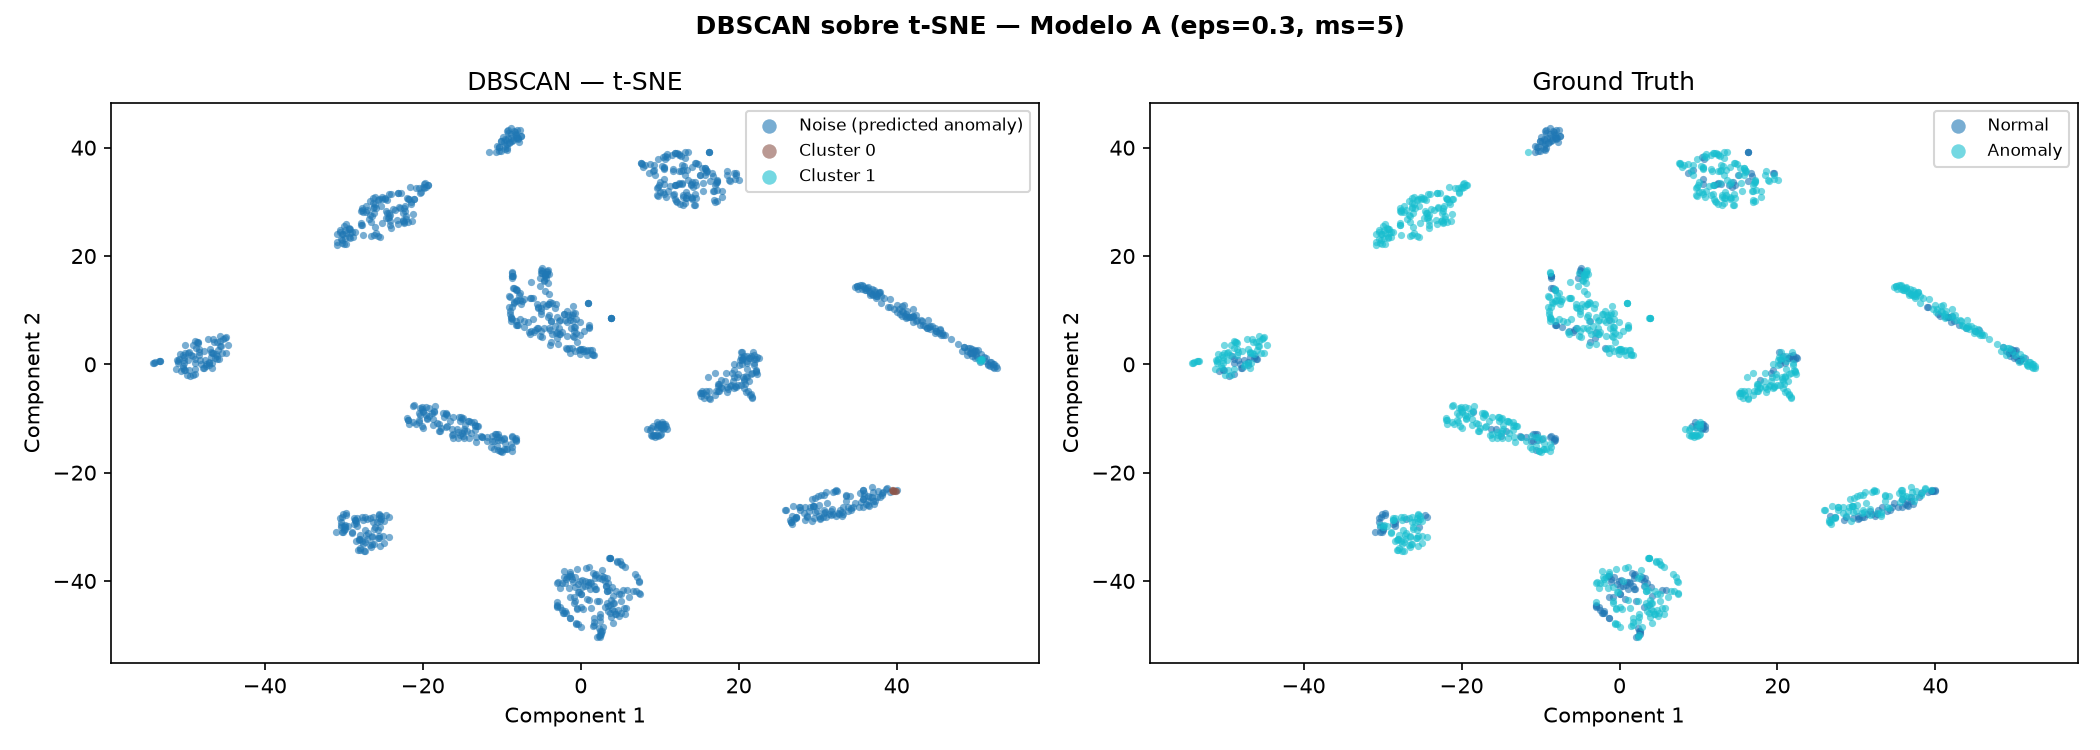
\includegraphics[width=\columnwidth]{dbscan_tsne_modelo_a.png}
  \caption{DBSCAN sobre t-SNE — Modelo A (mejor F1 en DBSCAN: 0.860). Rojo: ruido predicho;
           panel derecho muestra etiquetas reales de anomalía.}
  \label{fig:dbscan}
\end{figure}

% ─────────────────────────────────────────────────────────────────────────────
\section{Discusión}

\subsection{Impacto del destilado}

El Modelo B supera al Modelo A en AUROC (0.453 vs. 0.365) y en F1 (0.230 vs.
0.173), confirmando que el destilado de ResNet-18 produce representaciones más
informativas para detección de anomalías. La pérdida combinada
($\alpha \cdot \mathcal{L}_{CE} + \beta \cdot \mathcal{L}_{feat_1} + \gamma
\cdot \mathcal{L}_{feat_2}$) actúa como regularizador implícito, guiando al
student hacia un espacio de embeddings más estructurado que el entrenamiento
desde cero.

\subsection{Embeddings vs. error de reconstrucción}

El error de reconstrucción MSE del U-Net obtiene el mayor AUROC global (0.490),
superando a la distancia de Mahalanobis sobre embeddings en todos los modelos.
Esto sugiere que, bajo las condiciones experimentales de este trabajo (50 épocas
máximo), la señal directa de reconstrucción captura las desviaciones anómalas
de forma más robusta que el espacio latente comprimido, que aún no forma
distribuciones gaussianas perfectamente definidas por clase.

\subsection{Análisis de overfitting}

El \textit{EarlyStopping} fue efectivo en todos los modelos. El Modelo A
convergió más rápido (época 12) mientras que el Modelo B requirió más épocas
(época 30) gracias a la señal de destilado más compleja. El U-Net con
lr=$10^{-4}$ y features=[64,128,256,512] obtuvo el menor val\_loss (0.0046).

\subsection{DBSCAN: PCA vs. t-SNE}

t-SNE produce separaciones notablemente superiores a PCA en todos los modelos.
Con PCA, ningún modelo genera clusters útiles para detección de anomalías
(F1 $< 0.09$, noise\_rate $< 5\%$). Con t-SNE, los tres modelos alcanzan
F1 $\approx$ 0.85--0.86 con noise\_rate $> 94\%$, lo que indica que casi
todos los puntos se clasifican como ruido. El Modelo A logra el mayor F1 (0.860)
con t-SNE, seguido de cerca por B (0.855) y C (0.846).

% ─────────────────────────────────────────────────────────────────────────────
\section{Conclusiones}

Este trabajo valida experimentalmente la hipótesis del destilado de modelos para
detección de anomalías. Los resultados principales son:

\begin{itemize}
  \item El Modelo B (destilado) supera al Modelo A (scratch) en AUROC
        (0.453 vs. 0.365) y F1 (0.230 vs. 0.173), validando que la
        transferencia de conocimiento de ResNet-18 mejora la calidad de
        los embeddings para detección de anomalías.
  \item El mejor detector global en AUROC es el error de reconstrucción
        del U-Net (0.490), superando a todos los métodos basados en
        embeddings con distancia de Mahalanobis.
  \item t-SNE produce separaciones muy superiores a PCA en DBSCAN
        (F1 $\approx$ 0.86 vs. $<$ 0.09), siendo el Modelo A el de
        mayor F1 (0.860), seguido de B (0.855) y C (0.846).
  \item El \textit{EarlyStopping} fue efectivo en todos los experimentos,
        evitando overfitting con convergencia entre las épocas 12 y 45
        según configuración.
\end{itemize}

Como trabajo futuro se propone explorar destilado a mayor profundidad
(\texttt{conv4\_x} y \texttt{conv5\_x}), destilado por respuesta con
temperatura adaptativa, y estrategias de detección multiescala para
anomalías de tamaño variable.

% ─────────────────────────────────────────────────────────────────────────────
\begin{thebibliography}{9}

\bibitem{bergmann2019mvtec}
P.~Bergmann, M.~Fauser, D.~Sattlegger, and C.~Steger,
``MVTec AD --- A Comprehensive Real-World Dataset for Unsupervised Anomaly Detection,''
\textit{CVPR}, 2019.

\bibitem{he2016deep}
K.~He, X.~Zhang, S.~Ren, and J.~Sun,
``Deep Residual Learning for Image Recognition,''
\textit{CVPR}, 2016.

\bibitem{hinton2015distilling}
G.~Hinton, O.~Vinyals, and J.~Dean,
``Distilling the Knowledge in a Neural Network,''
\textit{NIPS Deep Learning Workshop}, 2015.

\bibitem{ronneberger2015unet}
O.~Ronneberger, P.~Fischer, and T.~Brox,
``U-Net: Convolutional Networks for Biomedical Image Segmentation,''
\textit{MICCAI}, 2015.

\bibitem{lee2018simple}
K.~Lee, K.~Lee, H.~Lee, and J.~Shin,
``A Simple Unified Framework for Detecting Out-of-Distribution Samples and
Adversarial Attacks,''
\textit{NeurIPS}, 2018.

\end{thebibliography}

\end{document}
